% uWaterloo Thesis Template for LaTeX 
% Last Updated June 14, 2017 by Stephen Carr, IST Client Services
% FOR ASSISTANCE, please send mail to rt-IST-CSmathsci@ist.uwaterloo.ca

% Effective October 2006, the University of Waterloo 
% requires electronic thesis submission. See the uWaterloo thesis regulations at
% https://uwaterloo.ca/graduate-studies/thesis.

% DON'T FORGET TO ADD YOUR OWN NAME AND TITLE in the "hyperref" package
% configuration below. THIS INFORMATION GETS EMBEDDED IN THE PDF FINAL PDF DOCUMENT.
% You can view the information if you view Properties of the PDF document.

% Many faculties/departments also require one or more printed
% copies. This template attempts to satisfy both types of output. 
% It is based on the standard "book" document class which provides all necessary 
% sectioning structures and allows multi-part theses.

% DISCLAIMER
% To the best of our knowledge, this template satisfies the current uWaterloo requirements.
% However, it is your responsibility to assure that you have met all 
% requirements of the University and your particular department.
% Many thanks for the feedback from many graduates that assisted the development of this template.

% -----------------------------------------------------------------------

% By default, output is produced that is geared toward generating a PDF 
% version optimized for viewing on an electronic display, including 
% hyperlinks within the PDF.
 
% E.g. to process a thesis called "mythesis.tex" based on this template, run:

% pdflatex mythesis	-- first pass of the pdflatex processor
% bibtex mythesis	-- generates bibliography from .bib data file(s)
% makeindex         -- should be run only if an index is used 
% pdflatex mythesis	-- fixes numbering in cross-references, bibliographic references, glossaries, index, etc.
% pdflatex mythesis	-- fixes numbering in cross-references, bibliographic references, glossaries, index, etc.

% If you use the recommended LaTeX editor, Texmaker, you would open the mythesis.tex
% file, then click the PDFLaTeX button. Then run BibTeX (under the Tools menu).
% Then click the PDFLaTeX button two more times. If you have an index as well,
% you'll need to run MakeIndex from the Tools menu as well, before running pdflatex
% the last two times.

% N.B. The "pdftex" program allows graphics in the following formats to be
% included with the "\includegraphics" command: PNG, PDF, JPEG, TIFF
% Tip 1: Generate your figures and photos in the size you want them to appear
% in your thesis, rather than scaling them with \includegraphics options.
% Tip 2: Any drawings you do should be in scalable vector graphic formats:
% SVG, PNG, WMF, EPS and then converted to PNG or PDF, so they are scalable in
% the final PDF as well.
% Tip 3: Photographs should be cropped and compressed so as not to be too large.

% To create a PDF output that is optimized for double-sided printing: 
%
% 1) comment-out the \documentclass statement in the preamble below, and
% un-comment the second \documentclass line.
%
% 2) change the value assigned below to the boolean variable
% "PrintVersion" from "false" to "true".

% --------------------- Start of Document Preamble -----------------------

% Specify the document class, default style attributes, and page dimensions
% For hyperlinked PDF, suitable for viewing on a computer, use this:
\documentclass[letterpaper,12pt,titlepage,oneside,final]{book}
 
% For PDF, suitable for double-sided printing, change the PrintVersion variable below
% to "true" and use this \documentclass line instead of the one above:
%\documentclass[letterpaper,12pt,titlepage,openright,twoside,final]{book}

% Some LaTeX commands I define for my own nomenclature.
% If you have to, it's better to change nomenclature once here than in a 
% million places throughout your thesis!
\newcommand{\package}[1]{\textbf{#1}} % package names in bold text
\newcommand{\cmmd}[1]{\textbackslash\texttt{#1}} % command name in tt font 
\newcommand{\href}[1]{#1} % does nothing, but defines the command so the
    % print-optimized version will ignore \href tags (redefined by hyperref pkg).
%\newcommand{\texorpdfstring}[2]{#1} % does nothing, but defines the command
% Anything defined here may be redefined by packages added below...

% This package allows if-then-else control structures.
\usepackage{ifthen}
\newboolean{PrintVersion}
\setboolean{PrintVersion}{false} 
% CHANGE THIS VALUE TO "true" as necessary, to improve printed results for hard copies
% by overriding some options of the hyperref package below.

%\usepackage{nomencl} % For a nomenclature (optional; available from ctan.org)
\usepackage{amsmath,amssymb,amstext} % Lots of math symbols and environments
\usepackage[pdftex]{graphicx} % For including graphics N.B. pdftex graphics driver 

% Hyperlinks make it very easy to navigate an electronic document.
% In addition, this is where you should specify the thesis title
% and author as they appear in the properties of the PDF document.
% Use the "hyperref" package 
% N.B. HYPERREF MUST BE THE LAST PACKAGE LOADED; ADD ADDITIONAL PKGS ABOVE
\usepackage[pdftex,pagebackref=false]{hyperref} % with basic options
		% N.B. pagebackref=true provides links back from the References to the body text. This can cause trouble for printing.
\hypersetup{
    plainpages=false,       % needed if Roman numbers in frontpages
    unicode=false,          % non-Latin characters in Acrobat’s bookmarks
    pdftoolbar=true,        % show Acrobat’s toolbar?
    pdfmenubar=true,        % show Acrobat’s menu?
    pdffitwindow=false,     % window fit to page when opened
    pdfstartview={FitH},    % fits the width of the page to the window
    pdftitle={Stylistic\ Variation\ in\ Linguistics\ using\ Disentangled\ Latent\ Spaces},    % title: CHANGE THIS TEXT!
    pdfauthor={Vineet John},    % author: CHANGE THIS TEXT! and uncomment this line
    pdfsubject={Natural Language Processing},  % subject: CHANGE THIS TEXT! and uncomment this line
%    pdfkeywords={keyword1} {key2} {key3}, % list of keywords, and uncomment this line if desired
    pdfnewwindow=true,      % links in new window
    colorlinks=true,        % false: boxed links; true: colored links
    linkcolor=blue,         % color of internal links
    citecolor=green,        % color of links to bibliography
    filecolor=magenta,      % color of file links
    urlcolor=cyan           % color of external links
}
\ifthenelse{\boolean{PrintVersion}}{   % for improved print quality, change some hyperref options
\hypersetup{	% override some previously defined hyperref options
%    colorlinks,%
    citecolor=black,%
    filecolor=black,%
    linkcolor=black,%
    urlcolor=black}
}{} % end of ifthenelse (no else)

\usepackage[automake,toc,abbreviations]{glossaries-extra} % Exception to the rule of hyperref being the last add-on package
% If glossaries-extra is not in your LaTeX distribution, get it from CTAN (http://ctan.org/pkg/glossaries-extra), 
% although it's supposed to be in both the TeX Live and MikTeX distributions. There are also documentation and 
% installation instructions there.

% Setting up the page margins...
% uWaterloo thesis requirements specify a minimum of 1 inch (72pt) margin at the
% top, bottom, and outside page edges and a 1.125 in. (81pt) gutter
% margin (on binding side). While this is not an issue for electronic
% viewing, a PDF may be printed, and so we have the same page layout for
% both printed and electronic versions, we leave the gutter margin in.
% Set margins to minimum permitted by uWaterloo thesis regulations:
\setlength{\marginparwidth}{0pt} % width of margin notes
% N.B. If margin notes are used, you must adjust \textwidth, \marginparwidth
% and \marginparsep so that the space left between the margin notes and page
% edge is less than 15 mm (0.6 in.)
\setlength{\marginparsep}{0pt} % width of space between body text and margin notes
\setlength{\evensidemargin}{0.125in} % Adds 1/8 in. to binding side of all 
% even-numbered pages when the "twoside" printing option is selected
\setlength{\oddsidemargin}{0.125in} % Adds 1/8 in. to the left of all pages
% when "oneside" printing is selected, and to the left of all odd-numbered
% pages when "twoside" printing is selected
\setlength{\textwidth}{6.375in} % assuming US letter paper (8.5 in. x 11 in.) and 
% side margins as above
\raggedbottom

% The following statement specifies the amount of space between
% paragraphs. Other reasonable specifications are \bigskipamount and \smallskipamount.
\setlength{\parskip}{\medskipamount}

% The following statement controls the line spacing.  The default
% spacing corresponds to good typographic conventions and only slight
% changes (e.g., perhaps "1.2"), if any, should be made.
\renewcommand{\baselinestretch}{1} % this is the default line space setting

% By default, each chapter will start on a recto (right-hand side)
% page.  We also force each section of the front pages to start on 
% a recto page by inserting \cleardoublepage commands.
% In many cases, this will require that the verso page be
% blank and, while it should be counted, a page number should not be
% printed.  The following statements ensure a page number is not
% printed on an otherwise blank verso page.
\let\origdoublepage\cleardoublepage
\newcommand{\clearemptydoublepage}{%
  \clearpage{\pagestyle{empty}\origdoublepage}}
\let\cleardoublepage\clearemptydoublepage

% Define Glossary terms (This is properly done here, in the preamble. Could be \input{} from a file...)
% Main glossary entries -- definitions of relevant terminology
 
\makeglossaries

%======================================================================
%   L O G I C A L    D O C U M E N T -- the content of your thesis
%======================================================================
\begin{document}

% For a large document, it is a good idea to divide your thesis
% into several files, each one containing one chapter.
% To illustrate this idea, the "front pages" (i.e., title page,
% declaration, borrowers' page, abstract, acknowledgements,
% dedication, table of contents, list of tables, list of figures,
% nomenclature) are contained within the file "uw-ethesis-frontpgs.tex" which is
% included into the document by the following statement.
%----------------------------------------------------------------------
% FRONT MATERIAL
%----------------------------------------------------------------------
% T I T L E   P A G E
% -------------------
% Last updated June 14, 2017, by Stephen Carr, IST-Client Services
% The title page is counted as page `i' but we need to suppress the
% page number. Also, we don't want any headers or footers.
\pagestyle{empty}
\pagenumbering{roman}

% The contents of the title page are specified in the "titlepage"
% environment.
\begin{titlepage}
        \begin{center}
        \vspace*{1.0cm}

        \Huge
        {\bf University of Waterloo E-Thesis Template for \LaTeX }

        \vspace*{1.0cm}

        \normalsize
        by \\

        \vspace*{1.0cm}

        \Large
        Pat Neugraad \\

        \vspace*{3.0cm}

        \normalsize
        A thesis \\
        presented to the University of Waterloo \\ 
        in fulfillment of the \\
        thesis requirement for the degree of \\
        Doctor of Philosophy \\
        in \\
        Zoology \\

        \vspace*{2.0cm}

        Waterloo, Ontario, Canada, 2017 \\

        \vspace*{1.0cm}

        \copyright\ Pat Neugraad 2017 \\
        \end{center}
\end{titlepage}

% The rest of the front pages should contain no headers and be numbered using Roman numerals starting with `ii'
\pagestyle{plain}
\setcounter{page}{2}

\cleardoublepage % Ends the current page and causes all figures and tables that have so far appeared in the input to be printed.
% In a two-sided printing style, it also makes the next page a right-hand (odd-numbered) page, producing a blank page if necessary.

 
% E X A M I N I N G   C O M M I T T E E (Required for Ph.D. theses only)
% Remove or comment out the lines below to remove this page
\begin{center}\textbf{Examining Committee Membership}\end{center}
  \noindent
The following served on the Examining Committee for this thesis. The decision of the Examining Committee is by majority vote.
  \bigskip
  
  \noindent
\begin{tabbing}
Internal-External Member: \=  \kill % using longest text to define tab length
External Examiner: \>  Bruce Bruce \\ 
\> Professor, Dept. of Philosophy of Zoology, University of Wallamaloo \\
\end{tabbing} 
  \bigskip
  
  \noindent
\begin{tabbing}
Internal-External Member: \=  \kill % using longest text to define tab length
Supervisor(s): \> Doris Johnson \\
\> Professor, Dept. of Zoology, University of Waterloo \\
\> Andrea Anaconda \\
\> Professor Emeritus, Dept. of Zoology, University of Waterloo \\
\end{tabbing}
  \bigskip
  
  \noindent
  \begin{tabbing}
Internal-External Member: \=  \kill % using longest text to define tab length
Internal Member: \> Pamela Python \\
\> Professor, Dept. of Zoology, University of Waterloo \\
\end{tabbing}
  \bigskip
  
  \noindent
\begin{tabbing}
Internal-External Member: \=  \kill % using longest text to define tab length
Internal-External Member: \> Deepa Thotta \\
\> Professor, Dept. of Philosophy, University of Waterloo \\
\end{tabbing}
  \bigskip
  
  \noindent
\begin{tabbing}
Internal-External Member: \=  \kill % using longest text to define tab length
Other Member(s): \> Leeping Fang \\
\> Professor, Dept. of Fine Art, University of Waterloo \\
\end{tabbing}

\cleardoublepage

% D E C L A R A T I O N   P A G E
% -------------------------------
  % The following is a sample Delaration Page as provided by the GSO
  % December 13th, 2006.  It is designed for an electronic thesis.
  \noindent
I hereby declare that I am the sole author of this thesis. This is a true copy of the thesis, including any required final revisions, as accepted by my examiners.

  \bigskip
  
  \noindent
I understand that my thesis may be made electronically available to the public.

\cleardoublepage

% A B S T R A C T
% ---------------

\begin{center}\textbf{Abstract}\end{center}

This is the abstract.

Vulputate minim vel consequat praesent at vel iusto et, ex delenit, esse euismod luptatum augue ut sit et eu vel augue autem feugiat, quis ad dolore. Nulla vel, laoreet lobortis te commodo elit qui aliquam enim ex iriure ea ullamcorper nostrud lorem, lorem laoreet eu ex ut vel in zzril wisi quis. Nisl in autem praesent dignissim, sit vel aliquam at te, vero dolor molestie consequat.

Tation iriure sed wisi feugait odio dolore illum duis in accumsan velit illum consequat consequat ipsum molestie duis duis ut ullamcorper. Duis exerci odio blandit vero dolore eros odio amet et nisl in nostrud consequat iusto eum suscipit autem vero. Iusto dolore exerci, ut erat ex, magna in facilisis duis amet feugait augue accumsan zzril delenit aliquip dignissim at. Nisl molestie nibh, vulputate feugait nibh luptatum ea delenit nostrud dolore minim veniam odio volutpat delenit nulla accumsan eum vero ullamcorper eum. Augue velit veniam, dolor, exerci ea feugiat nulla molestie, veniam nonummy nulla dolore tincidunt, consectetuer dolore nulla ipsum commodo.

At nostrud lorem, lorem laoreet eu ex ut vel in zzril wisi. Suscipit consequat in autem praesent dignissim, sit vel aliquam at te, vero dolor molestie consequat eros tation facilisi diam dolor. Odio luptatum dolor in facilisis et facilisi et adipiscing suscipit eu iusto praesent enim, euismod consectetuer feugait duis. Odio veniam et iriure ad qui nonummy aliquip at qui augue quis vel diam, nulla. Autem exerci tation iusto, hendrerit et, tation esse consequat ut velit te dignissim eu esse eros facilisis lobortis, lobortis hendrerit esse dignissim nisl. Nibh nulla minim vel consequat praesent at vel iusto et, ex delenit, esse euismod luptatum.

Ut eum vero ullamcorper eum ad velit veniam, dolor, exerci ea feugiat nulla molestie, veniam nonummy nulla. Elit tincidunt, consectetuer dolore nulla ipsum commodo, ut, at qui blandit suscipit accumsan feugiat vel praesent. In dolor, ea elit suscipit nisl blandit hendrerit zzril. Sit enim, et dolore blandit illum enim duis feugiat velit consequat iriure sed wisi feugait odio dolore illum duis. Et accumsan velit illum consequat consequat ipsum molestie duis duis ut ullamcorper nulla exerci odio blandit vero dolore eros odio amet et.

In augue quis vel diam, nulla dolore exerci tation iusto, hendrerit et, tation esse consequat ut velit. Duis dignissim eu esse eros facilisis lobortis, lobortis hendrerit esse dignissim nisl illum nulla minim vel consequat praesent at vel iusto et, ex delenit, esse euismod. Nulla augue ut sit et eu vel augue autem feugiat, quis ad dolore te vel, laoreet lobortis te commodo elit qui aliquam enim ex iriure. Ut ullamcorper nostrud lorem, lorem laoreet eu ex ut vel in zzril wisi quis consequat in autem praesent dignissim, sit vel. Dolore at te, vero dolor molestie consequat eros tation facilisi diam. Feugait augue luptatum dolor in facilisis et facilisi et adipiscing suscipit eu iusto praesent enim, euismod consectetuer feugait duis vulputate veniam et.

Ad eros odio amet et nisl in nostrud consequat iusto eum suscipit autem vero enim dolore exerci, ut. Esse ex, magna in facilisis duis amet feugait augue accumsan zzril. Lobortis aliquip dignissim at, in molestie nibh, vulputate feugait nibh luptatum ea delenit nostrud dolore minim veniam odio. Euismod delenit nulla accumsan eum vero ullamcorper eum ad velit veniam. Quis, exerci ea feugiat nulla molestie, veniam nonummy nulla. Elit tincidunt, consectetuer dolore nulla ipsum commodo, ut, at qui blandit suscipit accumsan feugiat vel praesent.

Dolor zzril wisi quis consequat in autem praesent dignissim, sit vel aliquam at te, vero. Duis molestie consequat eros tation facilisi diam dolor augue. Dolore dolor in facilisis et facilisi et adipiscing suscipit eu iusto praesent enim, euismod consectetuer feugait duis vulputate.

\cleardoublepage

% A C K N O W L E D G E M E N T S
% -------------------------------

\begin{center}\textbf{Acknowledgements}\end{center}

I would like to thank all the little people who made this thesis possible.
\cleardoublepage

% D E D I C A T I O N
% -------------------

\begin{center}\textbf{Dedication}\end{center}

This is dedicated to the one I love.
\cleardoublepage

% T A B L E   O F   C O N T E N T S
% ---------------------------------
\renewcommand\contentsname{Table of Contents}
\tableofcontents
\cleardoublepage
\phantomsection    % allows hyperref to link to the correct page

% L I S T   O F   T A B L E S
% ---------------------------
\addcontentsline{toc}{chapter}{List of Tables}
\listoftables
\cleardoublepage
\phantomsection		% allows hyperref to link to the correct page

% L I S T   O F   F I G U R E S
% -----------------------------
\addcontentsline{toc}{chapter}{List of Figures}
\listoffigures
\cleardoublepage
\phantomsection		% allows hyperref to link to the correct page

% GLOSSARIES (Lists of definitions, abbreviations, symbols, etc. provided by the glossaries-extra package)
% -----------------------------
\printglossaries
\cleardoublepage
\phantomsection		% allows hyperref to link to the correct page

% Change page numbering back to Arabic numerals
\pagenumbering{arabic}



%----------------------------------------------------------------------
% MAIN BODY
%----------------------------------------------------------------------
% Because this is a short document, and to reduce the number of files
% needed for this template, the chapters are not separate
% documents as suggested above, but you get the idea. If they were
% separate documents, they would each start with the \chapter command, i.e, 
% do not contain \documentclass or \begin{document} and \end{document} commands.
%======================================================================
\chapter{Introduction}
%======================================================================


Natural Language Processing (NLP) is a sub-field of Artificial Intelligence (AI) that deals with the understanding and generation of human languages.

Recently many of the statistical NLP methods are giving way to neural models to parametrize more expressive models of language. This includes machine translation, dialogue modeling, abstractive summarization, document classification etc.

The problem this thesis attempts to tackle is the neural disentanglement of style and content in text to enable conditioned generation of text. This is analogous to style transfer in computer vision \cite{gatys2016image}. The formulation of the problem in the vision domain is to transfer the visual style from one image to the other, as illustrated in Figure \ref{fig:style-transfer-vision} \footnote{Images downloaded from \url{https://github.com/fzliu/style-transfer}}. Stylistic transfer in text is based on a similar premise, where, given a an arbitrary body of text and a predefined style governed by a set of attributes like sentiment, emotion, tense, authorship, a new body of text can be generated such that it incorporates all of the pre-defined attributes its generation is being conditioned on.

\begin{figure}[ht]
	\centering
	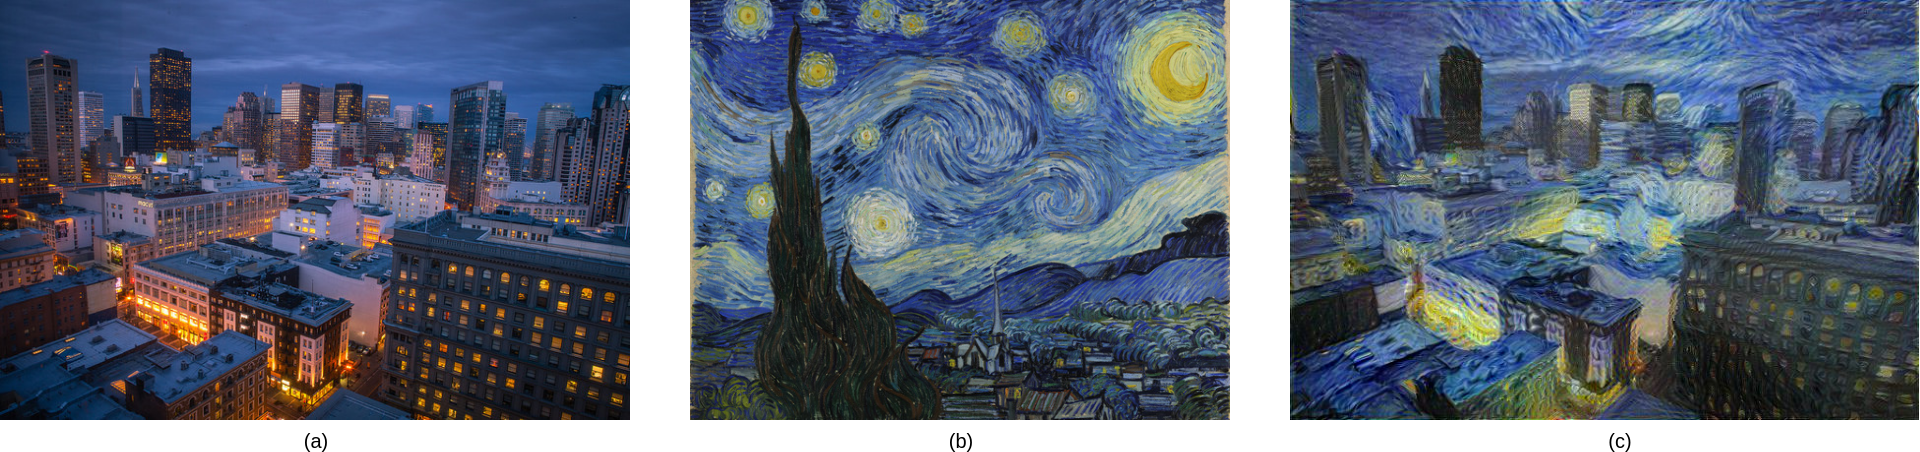
\includegraphics[width=.8\textwidth]{images/style-transfer-vision.png}
	\caption{\label{fig:style-transfer-vision}Sample of vision style transfer. Image (a) provides the content, image (b) provides the style and image (c) is the final generated image}
\end{figure}

This problem in the context of text was first introduced in 2012 \cite{xu2012paraphrasing} as a statistical model that attempted to paraphrase bodies of text in a different style using a simple replacement strategy. An few examples from this paper are shown in Table \ref{table:paraphrasing-for-style-results}. Since the overwhelming adopting of neural network based models in the language community, there have been many more works which break new ground in this area. These works will be described in detail in Section \ref{related-work-section}.

\begin{table}[ht]
	\centering
	\begin{tabular}{ | p{.45\linewidth} | p{.45\linewidth} | }
		\hline
		\textbf{Input}                                              & \textbf{Output}                                      \\
		\hline \hline
		i will bite thee by the ear for that jest .                 & i ’ ll bite you by the ear for that joke .           \\
		\hline
		what further woe conspires against mine age ?               & what ’ s true despair conspires against my old age ? \\
		\hline
		how doth my lady ?                                          & how is my lady ?                                     \\
		\hline
		hast thou slain tybalt ?                                    & have you killed tybalt ?                             \\
		\hline
		an i might live to see thee married once , i have my wish . & if i could live to see you married, i ’ ve my wish . \\
		\hline
		benvolio , who began this bloody fray ?                     & benvolio , who started this bloody fight itself ?    \\
		\hline
		what is your will ?                                         & what do you want ?                                   \\
		\hline
		call her forth to me .                                      & bring her out to me .                                \\
		\hline
	\end{tabular}
	\label{table:paraphrasing-for-style-results}
	\caption{Results of transferring authorship style from Shakespearan plays to modern english}
\end{table}

\section{Problem Statement}

The general problem statement the thesis tackles can be stated as exploratory foray into the previous approaches used for linguistic style transfer and also provides a novel approach to solve this open problem, and juxtaposes this approach and it's experimental results against the current state-of-the-art models.

%======================================================================
\chapter{Background}
%======================================================================

\section{Natural Language Generation}

Natural Language Generation (NLG) is a sub-field of Natural Language Processing that attempts to generate a sequence of words that resemble natural human languages. Traditionally, this can be done by either using production rules of a pre-defined grammar, or by performing statistical analyses of existing human-written texts to predict sequences of words based on their occurrence probabilities.

\section{Natural Language Understanding}

Natural Language Understanding (NLU) is another sub-field of Natural Language Processing which can be viewed as the converse of what is done in Natural Language Generation. Given a corpus of text, Natural Language Understanding is a collection of tasks that extract structured information from the text. A few examples of Natural Language Understanding tasks are sentiment analysis, emotion detection, entity-relation mapping, language comprehension etc.

\section{Recurrent Neural Networks}

Recurrent neural networks are a sub-class of artificial neural networks that can be considered a neural network equivalent to a Hidden Markov Model. Its units forms a directed graph that operates on a sequence of inputs when unrolled temporally. This makes them useful to extract features from arbitrary length sequences of input like audio or text.

\section{Sequence to Sequence Modeling}

This is a class of problems that models functions to map from one sequence to another. First introduced in \cite{sutskever2014sequence}, the general premise of sequence to sequence has been a flexible framework for modelling transformations made to arbitrary length sequences. In the natural language processing community, the main tasks that benefit from the encoder-decoder framework are neural machine translation, dialogue modeling, question answering for which there exists two distinct distributions of data, and the model is trained to learn the mapping from one to the other.


%======================================================================
\chapter{Related Work} \label{related-work-section}
%======================================================================


%======================================================================
\chapter{Challenges}
%======================================================================


%======================================================================
\chapter{Methods}
%======================================================================

%======================================================================
\chapter{Observations}
%======================================================================

This would be a good place for some figures and tables.


%----------------------------------------------------------------------
% END MATERIAL
%----------------------------------------------------------------------

% B I B L I O G R A P H Y
% -----------------------

% The following statement selects the style to use for references.  It controls the sort order of the entries in the bibliography and also the formatting for the in-text labels.
\bibliographystyle{plain}
% This specifies the location of the file containing the bibliographic information.  
% It assumes you're using BibTeX (if not, why not?).
\cleardoublepage % This is needed if the book class is used, to place the anchor in the correct page,
% because the bibliography will start on its own page.
% Use \clearpage instead if the document class uses the "oneside" argument
\phantomsection  % With hyperref package, enables hyperlinking from the table of contents to bibliography             
% The following statement causes the title "References" to be used for the bibliography section:
\renewcommand*{\bibname}{References}

% Add the References to the Table of Contents
\addcontentsline{toc}{chapter}{\textbf{References}}

\bibliography{uw-ethesis}
% Tip 5: You can create multiple .bib files to organize your references. 
% Just list them all in the \bibliogaphy command, separated by commas (no spaces).

% The following statement causes the specified references to be added to the bibliography% even if they were not 
% cited in the text. The asterisk is a wildcard that causes all entries in the bibliographic database to be included (optional).
\nocite{*}

\end{document}
